\part{Methods}
\label{pa:methods}
\chapter{Algorithms}
\section{Clustering}
To cluster or not to cluster is the question here. PPI networks already have
a great deal of edges and can be seen as clusters that we should not alter. On
the other hand, using clustering algorithms to make clusters out of
PPI-networks gives us the more control over the clusters and has the potential
to identify protein complexes\cite{ap-vs-mcl}. How big they should be, how many
of them we want, should we cluster on a certain attribute, or even several? We
have chosen to go with the \textit{Markov Cluster}(MCL)\cite{mcl} clustering
algorithm in \textit{clusterMaker2}, without any limitations to the amount of
clusters. We prototyped Ranklust with \textit{Affinity
Propagation}(AP)\cite{affinity-propagation} because of its ease of use and low
execution time, but it has been proven through a comparison between MCL and AP,
that concluded with MCL having better performance in many aspects when it came
to cluster unweighted (binary interactions) PPI networks\cite{ap-vs-mcl}. These
aspects being noise tolerance and more robust behaviour.

\section{Ranking clusters}
We have used five algorithms to rank the clusters, MAA, MAM, PR, PRWR and HITS.
The first two are simple algorithms that through addition or multiplication
calculates a cluster average score. The three others utilize network ranking
algorithms from the Java JUNG\cite{jung} library.

Every algorithm implemented in Ranklust for ranking clusters except HITS takes
node and/or edge scores as input for calculating the scores for each cluster.

\subsection{Multiple Attribute Additive Method (MAA)}
Multiple attribute additive method is the first algorithm implemented.  The user
has the option of choosing an unlimited amount of attributes from nodes and
edges.

It goes through all of the nodes in each cluster and sums up the number-
attributes the user chose. Each cluster is then ranked based on the average sum
in each cluster and ranked descending, with the highest ranking cluster as the
most likely prostate cancer biomarker cluster.

There is a question as to how to rank the edges in the cluster. We chose to rank
each edge as it is listed to the user in Cytoscape. So if it is listed only once
time in the edge table, it will only be scored additively once. This decision
was based on simplicity. To not represent the edge as something the user did not
define it as, or is unable to understand. Some clustering algorithms might
assign the same node or edge to several clusters, though this is not the case
with the algorithms we use in this thesis. Support for this is only implemented
by MAA and MAM, as they were implemented before a final decision on which
clustering algorithms should be used. If MAA/MAM discovers this special case of
several scores for a single node or edge, it will assign it the highest value.
The reason for leaving this feature in Ranklust is to have an example on how it
can be done, should it be a problem in the future.

\subsection{Multiple Attribute Multiplication Method (MAM)}
Multiple attribute multiplication method is to some degree redundant,
considering what exists from before in Ranklust. The only difference from MAA is
the scale the scores will be in. MAA adds the scores from each node and edge in
the cluster through addition, MAM does it with multiplication.

A problem that occurs with multiplication is calculating scores for clusters
that contain nodes with a score between 0 and 1, since the score would decrease
to such a degree that it would be difficult to work with when normalizing the
scores. The solution we have chosen for this is to make a new score from the
old score, and add 1.0 to it. This way, when the existing average score in the
cluster is multiplied with the new score, it will always increase, unless the
old value was 0.0, then it will stay the same. In the case of values above 1,
they will also be given an increase by 1.0 in order to keep it consistent if the
scores vary between 0 to \textit{n}. % TODO: discussion -> could be normalized

\subsection{PageRank (PR) and Personalized PageRank (PRWP)}
A Random Walks\cite{random-walks2} algorithm which used priors, called
seed-weighted random walks ranking \cite{sw-rwr}, proved to be effective at
prioritizing biomarker candidates. PageRank (PR) is an algorithm based on the
Random Walks principle, and it is contained inside the Java library
\textit{JUNG}\cite{jung}.  PR was previously used by Google to rank webpages
\cite{pagerank}.  Personalized PageRank (PRWP)\cite{pr-bio} is a modified
version of PR, where nodes and edges can be assigned a score prior to the PR's
traversal of the network. PR can have values assigned to the edges, but it does
not require any scores in order to rank clusters, which PRWP does. Personalized
PageRank is abbreviated PRWP because of the Java classname it has in the Java
JUNG library
- \textit{PageRankWithPriors}.

The difference between MAA and MAM compared to PR and PRWP is how the network is
scored. MAA and MAM calculates the score for each cluster by summing up the
attributes in edges and nodes according to the cluster attribute. PRWP scores
the current network regardless of the clustering attribute. 

MCL gives the option of creating a clustered network, which opens up the
possibility of working with two types of the same network, non-clustered and
clustered. They both have the clustering attribute in the network, edge and node
table, so that the ranking algorithms are able to score the clusters.  PRWP
scores the currently selected network in Cytoscape, resulting in the option of
scoring the non-clustered network or clustered network. The last option gives
the clustering algorithm a bigger impact on the score, because the clustered
network has perturbated edges between nodes that is not in the same cluster. MCL
in Cytoscape can show the "inter-cluster" connecting edges, which is the egdes
that was perturbed during clustering. This last option is a combination of the
two others. It will be visually close to the clustered network, but algorithms
that run on the network with inter-cluster edges will have the same result as
the network only containing the cluster attribute.

Implementation wise, there is also a difference in how the scores are stored in
the network after the algorithm is finished executing. All the scores are stored
in the nodes. To give information to the user about the scores the edges
received, each edge will display the total score for the cluster it is a member
of, just like the nodes.

\subsection{Hyperlink-Induced Topic Search}
Hyperlink-Induced Topic Search, HITS, an algorithm that is similar to PageRank,
was developed around the same time \cite{hits}\cite{hits-origin} and is also
contained within the Java JUNG library. HITS will not be used to calculate
cluster scores and ranks, due to the fact that it does not require any form of
weighting in nodes or edges. Though, it can be used in combination with other
ranking algorithms through the use of MAM or MAA. 

An example of this could be running PRWP with a score attribute, then HITS on
the same network. The next step would be to combine the two scores from PRWP and
HITS with MAA. Though, the idea of achieving novel information on network
biomarkers for prostate cancer through this workflow is pure speculation, and we
have chosen to use each ranking algorithm separately, in order to limit the
amount of datasets to analyze.

\subsection{PR, PRWP and HITS}
Because PR, PRWP and HITS rely on an alpha variable controlling the probability
of a reset in the traversal of the network. This "traversal reset" is
automatically triggered if the algorithm hits a node with no outgoing edges. As
the clustering algorithms might change the edges in the network, the outcome of
performing ranking on a cluster-created network, or a network with only
a cluster attribute to identify the clusters, can be potentially vastly
different. The alpha value parameter will be set to 0.775. This is because the
results from running the similar algorithm "seed-weighted random walks ranking"
was achieved with an alpha value of 0.7 \cite{sw-rwr}. There is a report of
Google having used a value of 0.85 \cite{pr-parameters} as the alpha value, so
the average of these two should provide for a alpha value to start with.

Another parameter for PR, PRWP and HITS is the iteration parameter. For each
iteration of these algorithms, they assign a value to each node. Performing
multiple iterations contribute to stabilize these values. In the previously
mentioned report from Google \cite{pr-parameters}, a \textit{n x n} matrix where
\textit{n} was about 25 billion, required about 50 - 100 iterations in order to
stabilize the node values. Iterations needed to stabilize increase with the size
of the network, therefore the iteration value to start with will be 100, should
it not take too long to calculate. It should be way more than needed, because
the size of the network used to test with contains about 1500 nodes and 1500
edges.


\chapter{Creation of Neo4J database} % Insert appendix links to the scripts!
\section{Data preparation}
We created a Neo4J database and used a slightly modified Cytoscape app to
communicate with it. Input to the database is a modified version of data. The
data started as a PPI file from the StringDB. The file had a size of 3,9GB and
consisted of interactions between two proteins. Each line had two Ensembl
Protein IDs (ENSP), the type of interaction, what direction the interaction went
in and a score for the interaction. 

\begin{verbatim}
item_id_a	item_id_b	mode	action	a_is_acting	score
9606.ENSP00000000233	9606.ENSP00000000233	binding		0	800
\end{verbatim}

Then we strip this file in order to get a file with just the ENSP IDs. One line
per ID.

\begin{verbatim}
ENSP00000000233
ENSP00000005340
\end{verbatim}

Next up is the conversion from protein IDs to gene IDs coupled with Entrez ID.
This information we got from UniProt through the stripped ENSP IDs. The file
with the data is formatted like this:

\begin{verbatim}
Entry	EnsembleID	    Gene names
P84085	ENSP00000000233	ARF5
\end{verbatim}

Then match the \textit{EnsembleID} from UniProt, which is a ENSP ID, to the
\textit{item\_id\_a} and \textit{item\_id\_b} data from StringDB (without the
9606.  prefix). Then combine the Entrez id, which is the \textit{Entry} from
UniProt with \textit{Gene names} with a square (\textit{\#}) between them as
a separator to make it easier to split them when creating Cypher and GraphML
import queries for Neo4J. This combination makes up a single gene, and each line
in the file we write this information to consist of two genes and a type of
binding between them. The type of binding is provided by the StringDB file
mentioned first in this section. % label and refer instead of mentioning it!

\section{Neo4J setup and data import}

\subsection{Setup}
Not much of a setup is needed to get the database up and running. Every setting
that was changed in testing and using the database was set in the
\textit{conf/neo4j-server.properties} file, located in the directory relative to
the Neo4J database installation.

The database
location does not need to be set up, but knowing the location of the data that
is saved in the Neo4J database is somewhat crucial when working with several
database instances.

\begin{verbatim}
org.neo4j.server.database.location=data/string_mini.db
org.neo4j.server.webserver.port=7474
\end{verbatim}

NB! That path is relative to the location the neo4j database is run from.

Turning authentication on/off is also smart for testing purposes. Communicating
with a Neo4J database instance that demands authentication also requires the
usage of the modified Cytoscape app \textit{CyNeo4J}. This is because the app
does support everything we need except from authenticating with a database. For
the database, this is just having a boolean value \textit{true}/\textit{false}.

\begin{verbatim}
dbms.security.auth_enabled=true
\end{verbatim}

\subsection{Import}
Importing data into Neo4J is not very mature at this point. You have the
possibility to just use Neo4J's query language, \textit{Cypher}. However,
importing the whole gene data from StringDB and UniProt combined takes a long
time in Cypher, even if the language is the native language to Neo4J. The
alternative we used was \textit{neo4j-shell-tools} \cite{neo4j-tools}. It is
easy to install and supports import with \textit{CSV}, \textit{Geoff} and
\textit{GraphML} filetypes. A GraphML import took under 1 minute on an old and
underperforming laptop with 4GB memory, 2GHz CPU and a 128GB SSD \cite{laptop}.
In comparison, the Cypher import took several hours, with the same amount of
data. Testing related to Neo4J was not done with CSV-files, because Cytoscape
does not support exporting data of a whole network to a CSV file, only partial
information. On the other hand, Cytoscape has great support for exporting data
of a whole network to a GraphML file.

The Python scripts initialized the Neo4J database with data created with either
GraphML or Cypher. Importing any of them result in the same type of data in the
database, but because of the heavily increased speed using GraphML over Cypher,
we used GraphML exclusively to initialize the database. The nodes are created
with the forementioned \textit{Entrez ID} as primary key and \textit{Gene name}
as the displayed name in the Neo4J GUI.

\chapter{Ranklust implementation}
The clustering algorithms used to produce the clusters to rank will be AP and
MCL.

The clustered network can be constructed with AP, a clustering algorithm
\cite{affinity-propagation}. AP clustering concentrates on the nodes in the
network that are binding the rest of them together. Using affinity propagation
for clustering will produce results that represent a grouping of nodes that are
coupled by seemingly unimportant nodes to most clustering algorithms. But the AP
algorithm is good at expressing nodes that are not highly connected to many
nodes, but rather the nodes that are binding other highly connected nodes
together. This results in bigger clusters that can be a target for methods that
cure cancer by severing the interaction between biomarker genes.

It is also discussed how AP performs versus Markov clustering \cite{ap-vs-mcl}.
And since Markov algorithm performs better on protein interaction, it will also
be used to cluster the networks. An analysis between the rankings that come from
the Markov and AP clusterings will be performed, which hopefully will give
concrete results as to the pro's and con's of each algorithm. Some questions
should be raised as the analysis is done. For example, is both of the algorithms
good, but have different uses, even if they are not directly involved with the
ranking done after the clustering?  Are either AP or Markov useless for
a particular type of ranking afterwards?

The information provided through the whole process from what type of nodes
(protein or gene), interaction between the nodes and what kind of biomarker we
want to identify are all factors that will have a great impact on how all of
this should be combined. The order of operations on the network will also effect
the result. For example, AP clustering may create a few big clusters and many
small ones. At this stage, the results will consist of the biggest clusters
constructed from AP clustering that has focus on pure connection between nodes
and not their attributes. At this point, the cluster ranking algorithm of
Ranklust will be run in order to produce a picture of potential biomarkers. This
picture is the first and simplest step that will be used as a result for an
analysis. The analysis in this thesis will focus on validating the cluster
ranking scores as ways of indicating potential biomarkers. 

\chapter{Interpreting Ranklust results}
This was done solely by Python scripting, from formatting the data retrieved
from databases in order to construct networks in Cytoscape, to cleaning the
results exported from Ranklust, and analyzing the cleaned data.

\section{Network creation}
The network was created with protein interaction data from iRefWeb
\cite{irefweb}. 

\begin{figure}[H]
    \centering
    \caption{iRefWeb network query}
    \label{fig:irefweb}
    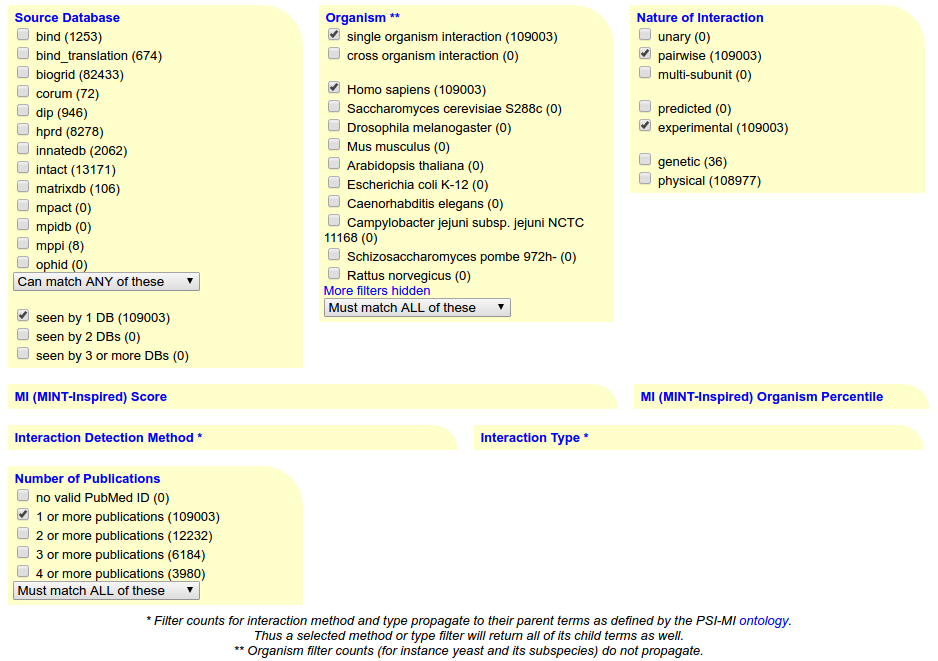
\includegraphics[width=15cm]{mitab_lite_109276}
\end{figure}

% change this from MITAB to MITAB-MINI!!!
It was downloaded in the MITAB format 
